\subsection{Vorüberlegungen}

\begin{defn}[kompakte topologische Mannigfaltigkeit]\label{defn:TopMan}
Ein kompakter Hausdorffraum $X$ heißt \emph{m-dimensionale kompakte topologische Mannigfaltigkeit}, wenn es stetige Abbildungen
\[ \theta_i: B^m \to X, ~i = 1, \dots, N \]
gibt (für ein $N \in \NN$), sodass gilt:
\begin{itemize}
	\item $\theta_i$ ist injektiv und $\theta_i^{-1}$ ist stetig sowie
	\item die Abbildung $\Theta: \bigcup_{i=1}^N(B^m,i) \to X: (r,i) \mapsto \theta_i(r)$ ist surjektiv.
\end{itemize}
Die Abbildungen $\theta_i$ bezeichnen wir als \emph{Karten}.
\end{defn}

\begin{prop}\label{prop:topManAlt}
Ist $X$ ein kompakter Hausdorffraum, so sind äquivalent:
\begin{enumerate}
	\item \label{prop:topManAlt:is}
		$X$ ist eine m-dimensionale kompakte topologische Mannigfaltigkeit.
	\item \label{prop:topManAlt:endl}
		Es gibt Abbildungen $\theta_i: B^m \to X$, sodass gilt:
		\begin{itemize}
			\item $\theta_i$ ist Homöomorphismus auf ihr Bild und
			\item $(\theta_i(B^m))_{i\in\{1,\dots,N\}}$ ist eine Überdeckung von $X$.
		\end{itemize}	\item \label{prop:topManAlt:pkt}
		Zu jedem $x \in X$ gibt es eine offene Umgebung $U_x \subseteq X$ von $x$ und einen Homöomorphismus $\theta_x: B^m \to U_x$, sodass $\theta_x(0) = x$.
	\item  \label{prop:topManAlt:abg}
		Es gibt Abbildungen $\theta_i: B^m \to X$, sodass gilt:
		\begin{itemize}
			\item $\theta_i$ ist Homöomorphismus auf ihr Bild und
			\item $(\theta_i(\overline{B_{0,5}^m}))_{i\in\{1,\dots,N\}}$ ist eine Überdeckung von $X$.
		\end{itemize}
\end{enumerate}
\end{prop}

\begin{proof}
\begin{itemize}
	\item[\ref*{prop:topManAlt:is}$\Rightarrow$\ref*{prop:topManAlt:endl}:] Die $\theta_i$ sind injektiv (also bijektiv auf ihr Bild) und stetig in beide Richtungen. Damit sind sie Homöomorphismen. Da $\Theta$ surjektiv ist, gibt es außerdem für jedes $x \in X$ ein $i \leq N$ und ein $r \in B^m$, sodass $x = \Theta(r,i) = \theta_i(r)$. Damit ist $(\theta_i(B^m))_{i\in\{1,\dots,N\}}$ eine Überdeckung.
	
	\item[\ref*{prop:topManAlt:is}$\Leftarrow$\ref*{prop:topManAlt:endl}:] Homöomorphismen sind insbesondere injektiv und in beide Richtungen stetig. Aus der Überdeckungseigenschaft folgt die Surjektivität von $\Theta$.
	
	\item[\ref*{prop:topManAlt:endl}$\Rightarrow$\ref*{prop:topManAlt:pkt}:] Sei $x \in X$. Da die $\theta_i(B^m)$ eine Überdeckung bilden, existiert ein $\theta_i$ mit $x \in \theta_i(B^m)$ und folglich $\theta_i^{-1}(x) \in B^m$. Weil $B^m$ offen ist, gibt es ein $\epsilon > 0$, sodass $B_\epsilon^m(\theta_i^{-1}(x)) \subseteq B^m$. Damit ist $U_x := \theta_i(B_\epsilon^m(\theta_i^{-1}(x)))$ eine offene Umgebung von $x$. Ferner ist die Abbildung
	\[\tau: B^m \to B_\epsilon^m(\theta_i^{-1}(x)): r \mapsto  \epsilon r + \theta_i^{-1}(x)\]
ein Homöomprphismus mit $\tau(0) = \theta_i^{-1}(x)$. Also ist $\theta_x := \theta_i \circ \tau: B^m \to U_x$ ein Homöomorphismus mit $\theta_x(0) = \theta_i \circ \tau(0) = \theta_i(\theta_i^{-1}(x)) = x$.
	
	\item[\ref*{prop:topManAlt:pkt}$\Rightarrow$\ref*{prop:topManAlt:abg}:] $(\theta_x(B_{0,5}^m))_{x\in X}$ ist Überdeckung von $X$. Da $X$ kompakt ist, gibt es also eine endliche Menge $M \subseteq X$, sodass auch $(\theta_x(B_{0,5}^m))_{x\in M}$ eine Überdeckung ist. Damit ist insbesondere auch $(\theta_x(\overline{B_{0,5}^m}))_{x\in M}$ eine Überdeckung von $X$ und es ist gezeigt, dass diese (endlich vielen) Abbildungen $\theta_x$ (für $x \in M$) die Anforderungen aus \ref*{prop:topManAlt:abg} erfüllen.

	\item[\ref*{prop:topManAlt:abg}$\Rightarrow$\ref*{prop:topManAlt:endl}:]Karten, die die Anforderungen aus \ref*{prop:topManAlt:abg} erfüllen, erfüllen offensichtlich insbesondere auch die aus \ref*{prop:topManAlt:endl}.	
\end{itemize}
\end{proof}

\begin{bem}
\cref*{prop:topManAlt:pkt} entspricht der üblichen Definition für kompakte topologische Mannigfaltigkeiten (die auch zur Definition von nicht notwendig kompakten topologischen Mannigfaltigkeiten verwendet wird).
\end{bem}

Die Klasse aller \komenTopMan{} mit stetigen Abbildungen als Morphismen bildet die \emph{Kategorie der kompakten topologischen Mannigfaltigkeiten} $\KatTopMan$. Da jede \komTopMan{} auch ein kompakter Hausdorffraum ist, ist $\KatTopMan$ offensichtlich eine Unterkategorie von $\KatTop$. 

Aufgrund der Gelfand-Dualität muss es folglich eine zu $\KatTopMan$ duale Unterkategorie von $\KatCAlg$ geben. Wir werden diese Kategorie als \emph{Kategorie der \CAlgMann} $\KatCAlgMan$ bezeichnen und im Folgenden versuchen die Objekte dieser Kategorie näher zu klassifizieren. Wir werden also versuchen die Frage zu beantworten, welche \CAlgn{} isomorph zum Raum der stetigen Funktionen über einer \komenTopMan{} sind.

Betrachten wir dazu eine \komTopMan{} $X$ mit Karten $\theta_i$. Über die Gelfand-Dualität erhalten wir zu $X$ die \CAlg{} $\stetig(X)$. Weiterhin erhalten wir aus den Karten von $X$ auf natürliche Weise stetige Algebrenhomomorphismen 
	\[k_i: \stetig(X) \to \stetig^b(B^m):= \{\varphi: B^m \to \CC ~|~ \varphi \text{ stetig und beschränkt}\}: \tau \mapsto \tau \circ\theta_i.\]
Die Eigenschaft solche \glqq Karten\grqq{} zu besitzen, bleibt offensichtlich unter Isomorphie erhalten (verknüpfe die Abbildungen mit dem Isomorphismus). Also müssen alle \CAlgn{} der Unterkategorie $\KatCAlgMan$ derartige \glqq Karten\grqq{} besitzen (wir werden diese im Folgenden als \emph{Algebrenkarten} bezeichnen). 

Nun sind die Karten einer \komTopMan{} jedoch nicht beliebige stetige Abbildungen, sondern sie besitzen zusätzlich noch eine Injektivitäts- und eine Surjektivitätseigenschaft. Diese Eigenschaften der Karten sollten sich in irgendeiner Weise auch in den Algebrenkarten widerspiegeln. 

Tatsächlich ist leicht zu sehen, dass sich aus der Surjektivität von $\Theta$, die Injektivität der Abbildung
	\[K: \stetig(X) \to (\stetig^b(B^m))^N: \tau \mapsto (\tau\circ\theta_1, \dots, \tau\circ\theta_N)\]
ergibt. 

Analog könnte man vielleicht erwarten, dass aus der Injektivität der Karten $\theta_i$ folgt, dass die Algebrenkarten $k_i$ surjektiv sind. Dass dies jedoch nicht der Fall ist, können wir an folgenden Beispiel sehen:

\begin{bsp}\label{bsp:ohneNS} $S^1 := \{z \in \CC ~|~ |z| = 1\}$ ist ein kompakter Hausdorffraum, der mit den Karten 
	\[\theta_{\hat{N}}: B^1 \to S^1: r \mapsto \exp{\pi i r - 0,5\pi i} \text{ und } \theta_{\hat{S}}: B^1 \to S^1: r \mapsto \exp{\pi i r + 0,5\pi i}\]
vollständig überdeckt wird. Also ist $S^1$ eine topologische Mannigfaltigkeit. Ferner ist die Abbildung:
	\[\varphi: B^1 \to \CC: r \mapsto r\]
offensichtlich stetig und beschränkt, d.h. $\varphi \in \stetig^b(B^1)$.

Wäre nun $k_{\hat{N}}: \stetig(S^1) \to \stetig^b(B^1): \tau \mapsto \tau \circ\theta_{\hat{N}}$ surjektiv, so müsste es eine Abbildung $\tau \in \stetig(S^1)$ geben, die auf $\varphi$ abgebildet wird. Dieses $\tau$ müsste dann aber direkt \glqq rechts\grqq{} von Nordpol fast $1$ und direkt \glqq links\grqq{} fast $-1$ sein - da $\tau$ stetig sein soll, hieße das:
	\begin{align*}
		1 &= \lim_{r\to 1}\varphi(r) = \lim_{r\to 1} \tau\circ\theta_{\hat{N}}(r) = \lim_{r\to 1}\tau(\exp{\pi i r - 0,5\pi i}) =  \tau(\exp{0,5\pi i}) = \\
		 &=\tau(\exp{-1,5\pi i}) = \lim_{r\to -1} \tau(\pi i r - 0,5\pi i) = \lim_{r\to -1} \tau\circ\theta_{\hat{N}}(r) = \lim_{r\to -1}\varphi(r) = -1
	\end{align*}
Also gibt es kein solches $\varphi$ und $k_{\hat{N}}$ ist nicht surjektiv.
\end{bsp}

\begin{figure}[h]
         \centering
         \begin{subfigure}[b]{0.3\textwidth}
                 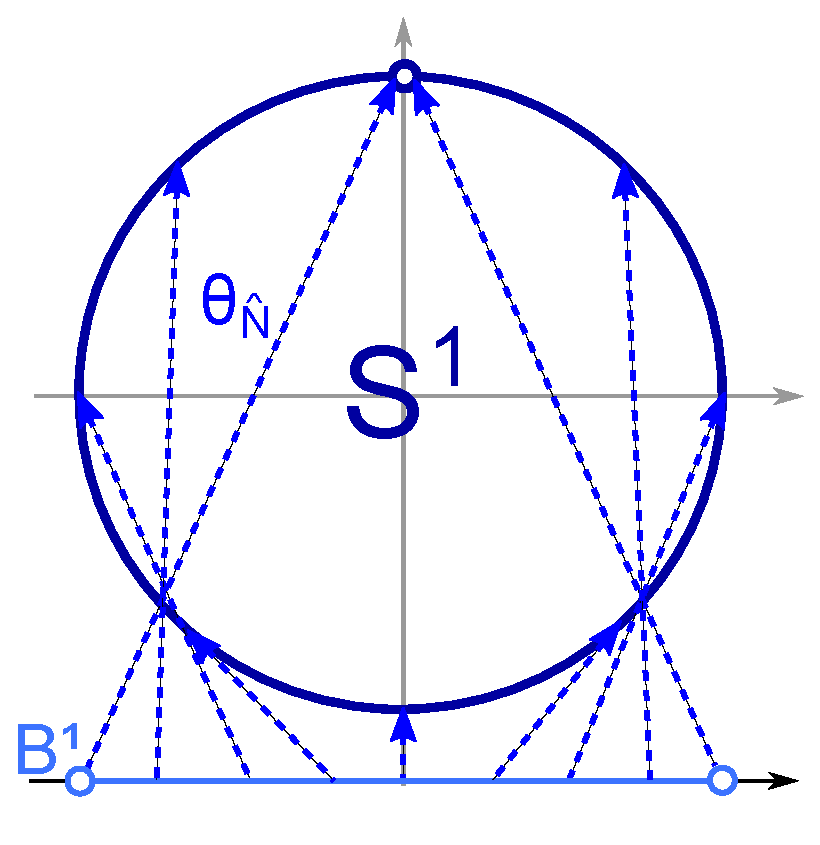
\includegraphics[width=\textwidth]{Bilder/keine-ueberdeckung.pdf}
                 \caption{\cref{bsp:ohneNS}}
         \end{subfigure}%
 			\qquad\qquad
         \begin{subfigure}[b]{0.3\textwidth}
                 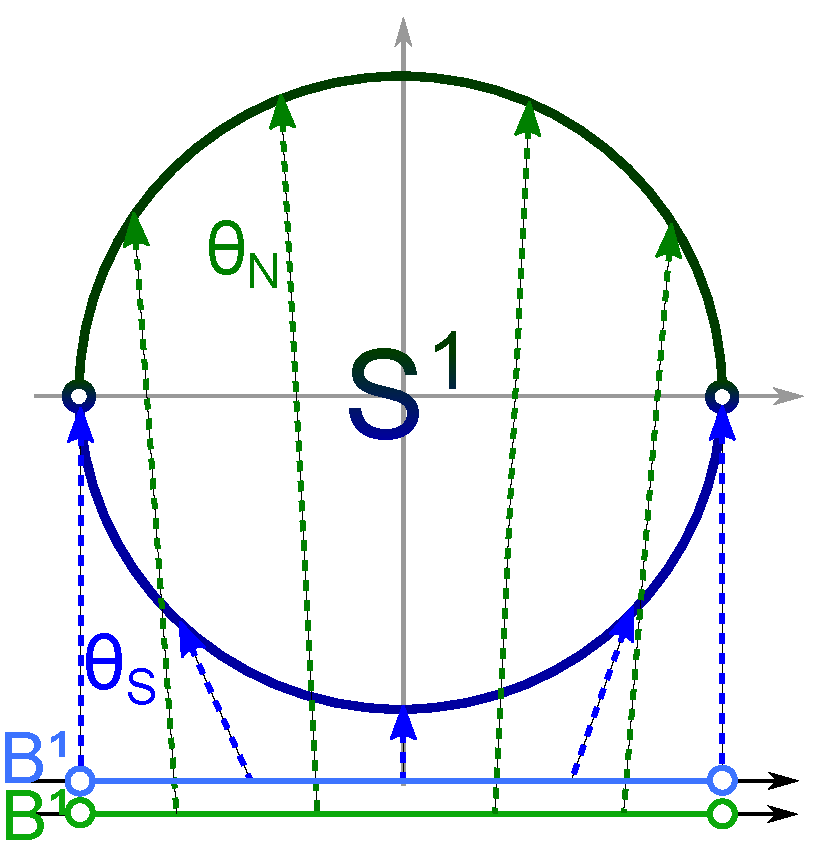
\includegraphics[width=\textwidth]{Bilder/ohne-aequator.pdf}
                 \caption{\cref{bsp:keine-Ueberdeckung}}
         \end{subfigure}
         \caption{Kartenabbildungen für $S^1$}
\end{figure}

Ein weiteres Problem ist, dass aus der Surjektivität von $\Theta$ zwar die Injektivität von $K$ folgt, nicht aber umgekehrt:

\begin{bsp}\label{bsp:keine-Ueberdeckung}Die Karten 
	\[\theta_S: B^1 \to S^1: r \mapsto \exp{0,5 \pi i (r-1)} \text{ und } \theta_N: B^1 \to S^1: r \mapsto \exp{0,5 \pi i (1-r)}\]
bilden keine vollständige Überdeckung von $S^1$ (die beiden Äquatorpunkte werden nicht getroffen). Dennoch wäre $K$ zu diesen Karten bereits injektiv. Denn gilt für zwei Abbildungen $\tau, \psi \in \stetig(S^1)$, dass $(\tau\circ\theta_S, \tau\circ\theta_N) = K(\tau) = K(\psi) = (\psi\circ\theta_S, \psi\circ\theta_N)$ ist, so können sich $\tau$ und $\psi$ höchstens noch an den Äquatorpunkten unterscheiden. Da $\tau$ und $\psi$ aber stetig sind, sind diese beiden Punkte bereits durch ihre Umgebung eindeutig festgelegt. Folglich müssen $\tau$ und $\psi$ auch hier übereinstimmen und sind damit identisch.
\end{bsp}

Insgesamt sehen wir also, dass die Surjektivität der Algebrenkarten eine zu starke Forderung ist, während die Injektivität von $K$ anscheinend eine zu schwache Bedingung ist. 